\section{Herramientas alternativas a DUJAL}
Previo al desarrollo del paquete, se hizo una investigación para buscar referencias acerca de otras herramientas similares a los componentes,
 tanto como para buscar inspiración, como para encontrar posibles limitaciones que paliar. A continuación se discute el estado del arte de algunos de los componentes más relevantes del paquete de herramientas.

\subsection{Sacudida de Cámara}
Las herramientas de sacudida de cámara o 'Screen Shake' no son demasiado populares o comunes en la Unity Asset Store\cite{unityAssetStore}, quizás se deba a la gran cantidad de tutoriales acerca del tema disponibles en 
todo internet. Sin embargo, tal y como evidencia un pequeño estudio desarrollado por Jump Trajectory: 'Screenshake that doesn’t suck'\cite{Screenshake}, la técnica utilizada por la mayoría de estos tutoriales es deficiente
y trae consigo serios problemas cuando se trabaja en espacios tridimensionales. El pricipal problema de estas es que al aplicar una traslación a una cámara en este tipo de espacios se puede provocar que dicha cámara acabe dentro 
de la geometría el nivel. Esto provoca un fenómeno conocido como 'clipping' (Figura \ref{fig:clipping}). Este problema se puede ver muy claramente en uno de los primeros resultados relacionados con la sacudida de cámara en la Unity Asset 
Store\cite{unityAssetStore}, el paquete de Camera Shake FX\cite{ShakeFX}. Otro de los paquetes más populares de sacudida de cámara es Camera Shake Pro\cite{ShakePro}, que pese a ser mucho más completo y no tener los problemas 
que presenta Jump Trajectory en su estudio, tampoco incluye una forma sencilla de definir curvas o líneas de animación que controlen la intensidad de la sacudidas. La implementación de DUJAL pretende incluir las observaciones 
de Jump Trajectory en su estudio, además de las funcionalidades de calidad de vida de Camera Shake Pro\cite{ShakePro} tales como traer prefabs que permitan tener al sistema funcionando en menos de dos minutos, tener 
efectos predefinidos que prescindan al usuario de tener que crear unos nuevos, o que la llamada al componente de sacudida sea una función estática y global para mayor facilidad de uso en el código. Además de incluir algunas
funcionalidades propias, como las previamente mencionadas curvas de animación que permitan crear infinitas sacudidas únicas de forma visual e intuitiva.

\begin{figure}[H]
    \centering
    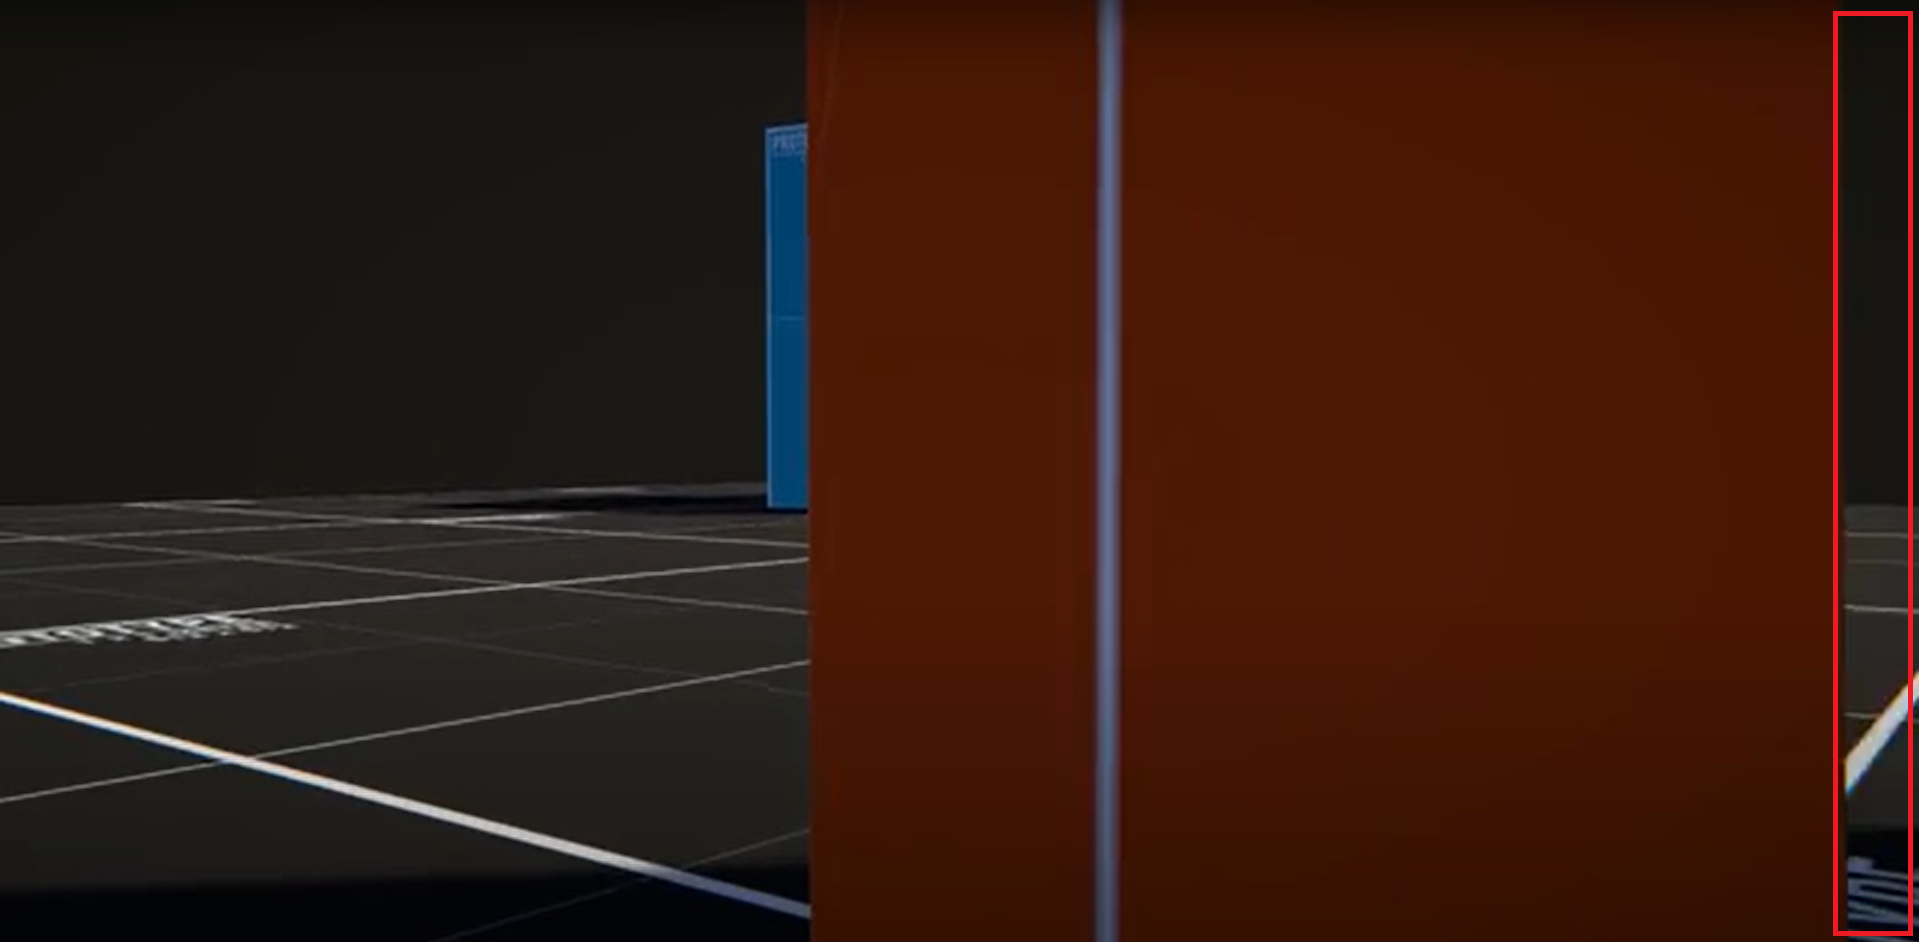
\includegraphics[width=350px,clip=true]{clipping.png}
    \caption{Representación del 'Cipping'}
    \label{fig:clipping}
\end{figure}

\subsection{Herramientas de Diálogos}
Con respecto a las herramientas de generación de diálogos hay una herramienta que es claramente el estándar, Dialogue System for Unity\cite{DialogueSystemUnity}, esta herramienta ha sido utilizada por algunos de los 
juegos más famosos de los últimos años, como Disco Elysium\cite{DiscoElysium} (Figura \ref{fig:discoelysium}) o 1000XRESIST\cite{1000xResist} (FIgura \ref{fig:1000xResist}). Es increíblemente completa dado que trae 
decenas de pequeñas herramientas para facilitar la implementación de diálogos en un juego. Permite exportar, guardar, modificar y localizar miles de textos de forma ligera y portable. El componente del Sistema de
 Diálogos de este proyecto se ha desarrollado usando esta herrameinta como referencia, con la diferencia de, en lugar de priorizar incluir los cientos de funcionalidades que forman parte de esta, priorizar la 
 facilidad de uso y la sencillez de la herramienta dado que ese es uno de los objetivos principales del proyecto. Dialogue System for Unity, aparte de ser menos accesible por ser de pago, requiere una inversión de 
 tiempo considerable para aprender a usarse, por otro lado, el componente creado para el proyecto se compone de una herramienta que permite traducir un esquema basado en grafos a un 'prefab' que se puede arrastrar 
 directamente a la escena de Unity y permite reproducir dicho diálogo sin necesidad de programar ni una sola línea de código.

\begin{figure}[H]
    \centering
    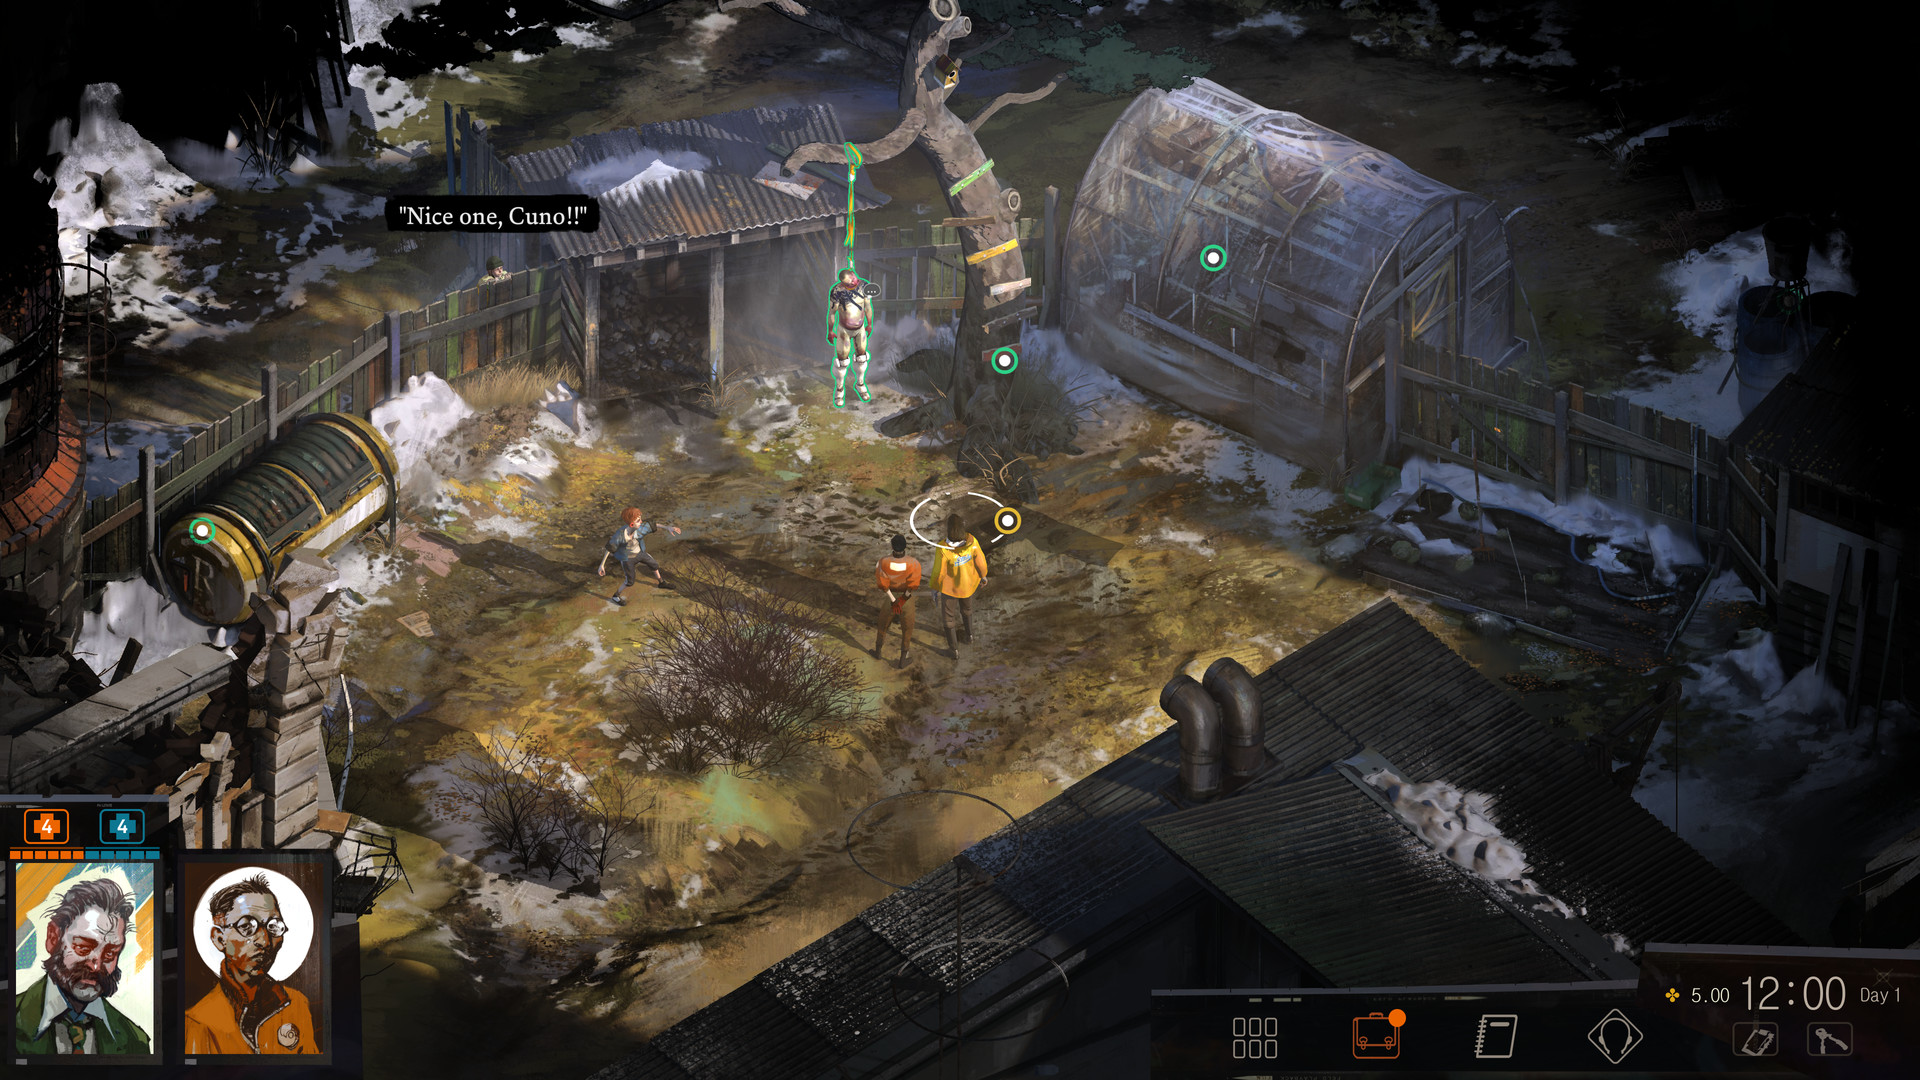
\includegraphics[width=350px,clip=true]{disco_elysium.png}
    \caption{Disco Elysium}
    \label{fig:discoelysium}
\end{figure}

\begin{figure}[H]
  \centering
  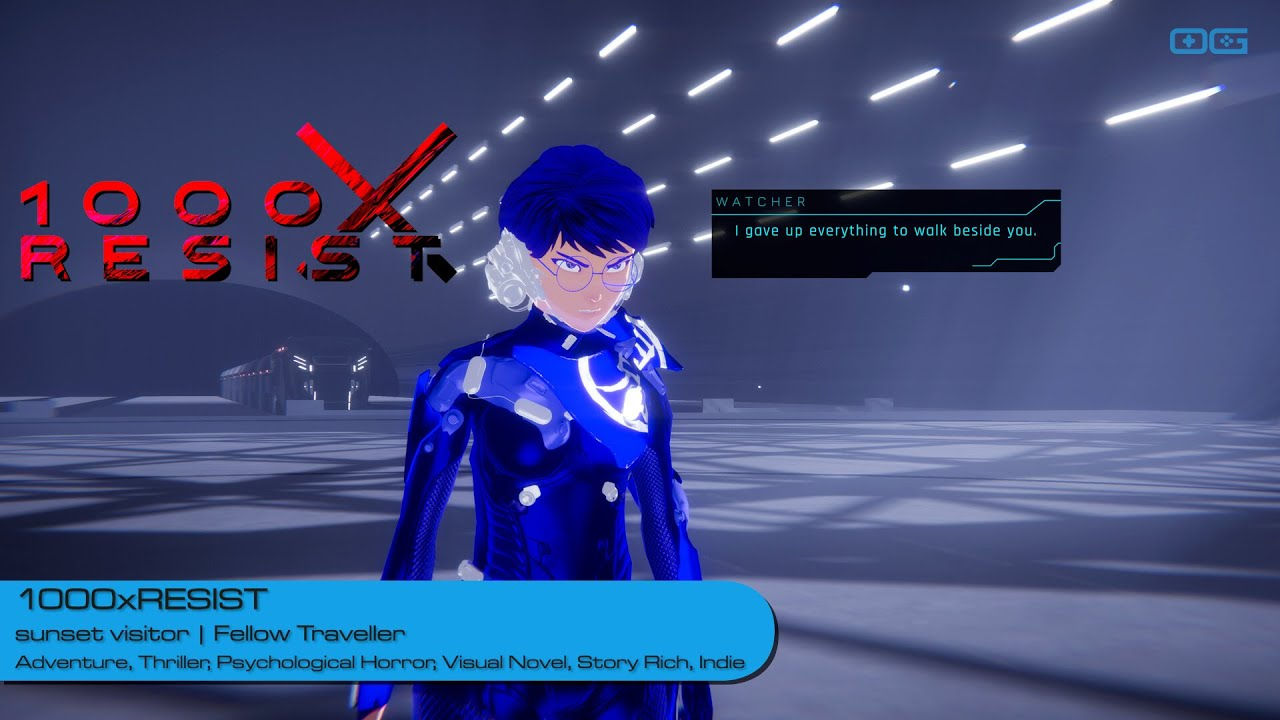
\includegraphics[width=350px,clip=true]{100xresist.png}
  \caption{1000xRESIST}
  \label{fig:1000xResist}
\end{figure}

 \subsection{Herramientas de Animación de Texto}
En lo referente a las animaciones de texto, hay una única herramienta que se corona como la más completa y profesional de todas, Text Animator\cite{TextAnimator}, desarrollada por febucci y utilizada en proyectos
 de gran envergadura, como Dredge (Figura \ref{fig:dredge}) o Cult of the Lamb (Figura \ref{fig:clamb}). Esta herramient permite añadir efectos a componentes Text Mesh Pro utilizando etiquetas similares a las de 
 Rich Text Format (<>). En estas se indica el tipo del efecto (<fade> Texto de Ejemplo </fade>), también admite modicadores de tiempo, intensidad o delay. La implementación de DUJAL es muy parecida, incluso utilizando 
 un formato muy similar a la hora de incluir efectos en el texto. La principal diferencia es que la estructura del procesado de efectos permite añadir, de forma sencilla y con una sintaxis muy parecida al scripting, 
 nuevos efectos a la librería de efectos del proyecto. Además, al ser un proyecto open source, es teóricamente sencillo publicar el código que permita añadir nuevos efectos a la librería.

\begin{figure}[H]
  \centering
  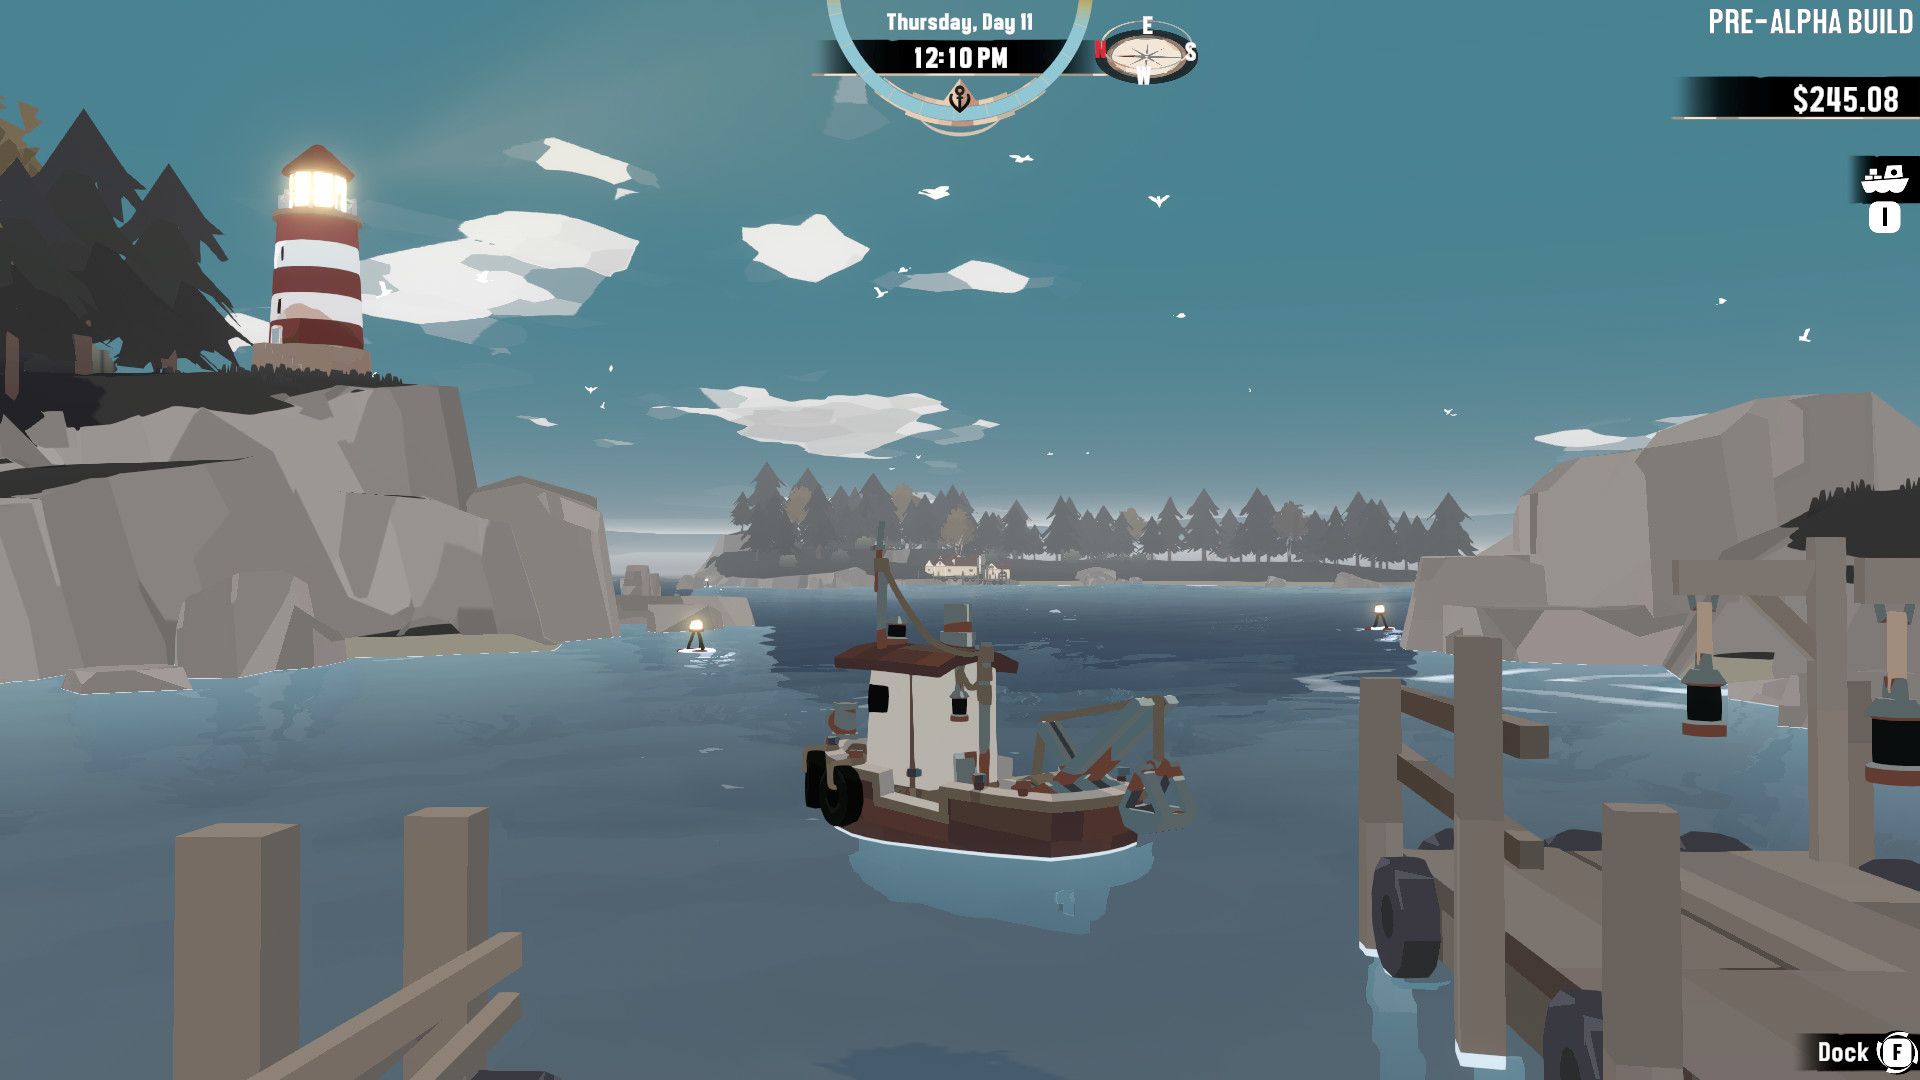
\includegraphics[width=350px,clip=true]{dredge.png}
  \caption{Dredge}
  \label{fig:dredge}
\end{figure}

\begin{figure}[H]
    \centering
    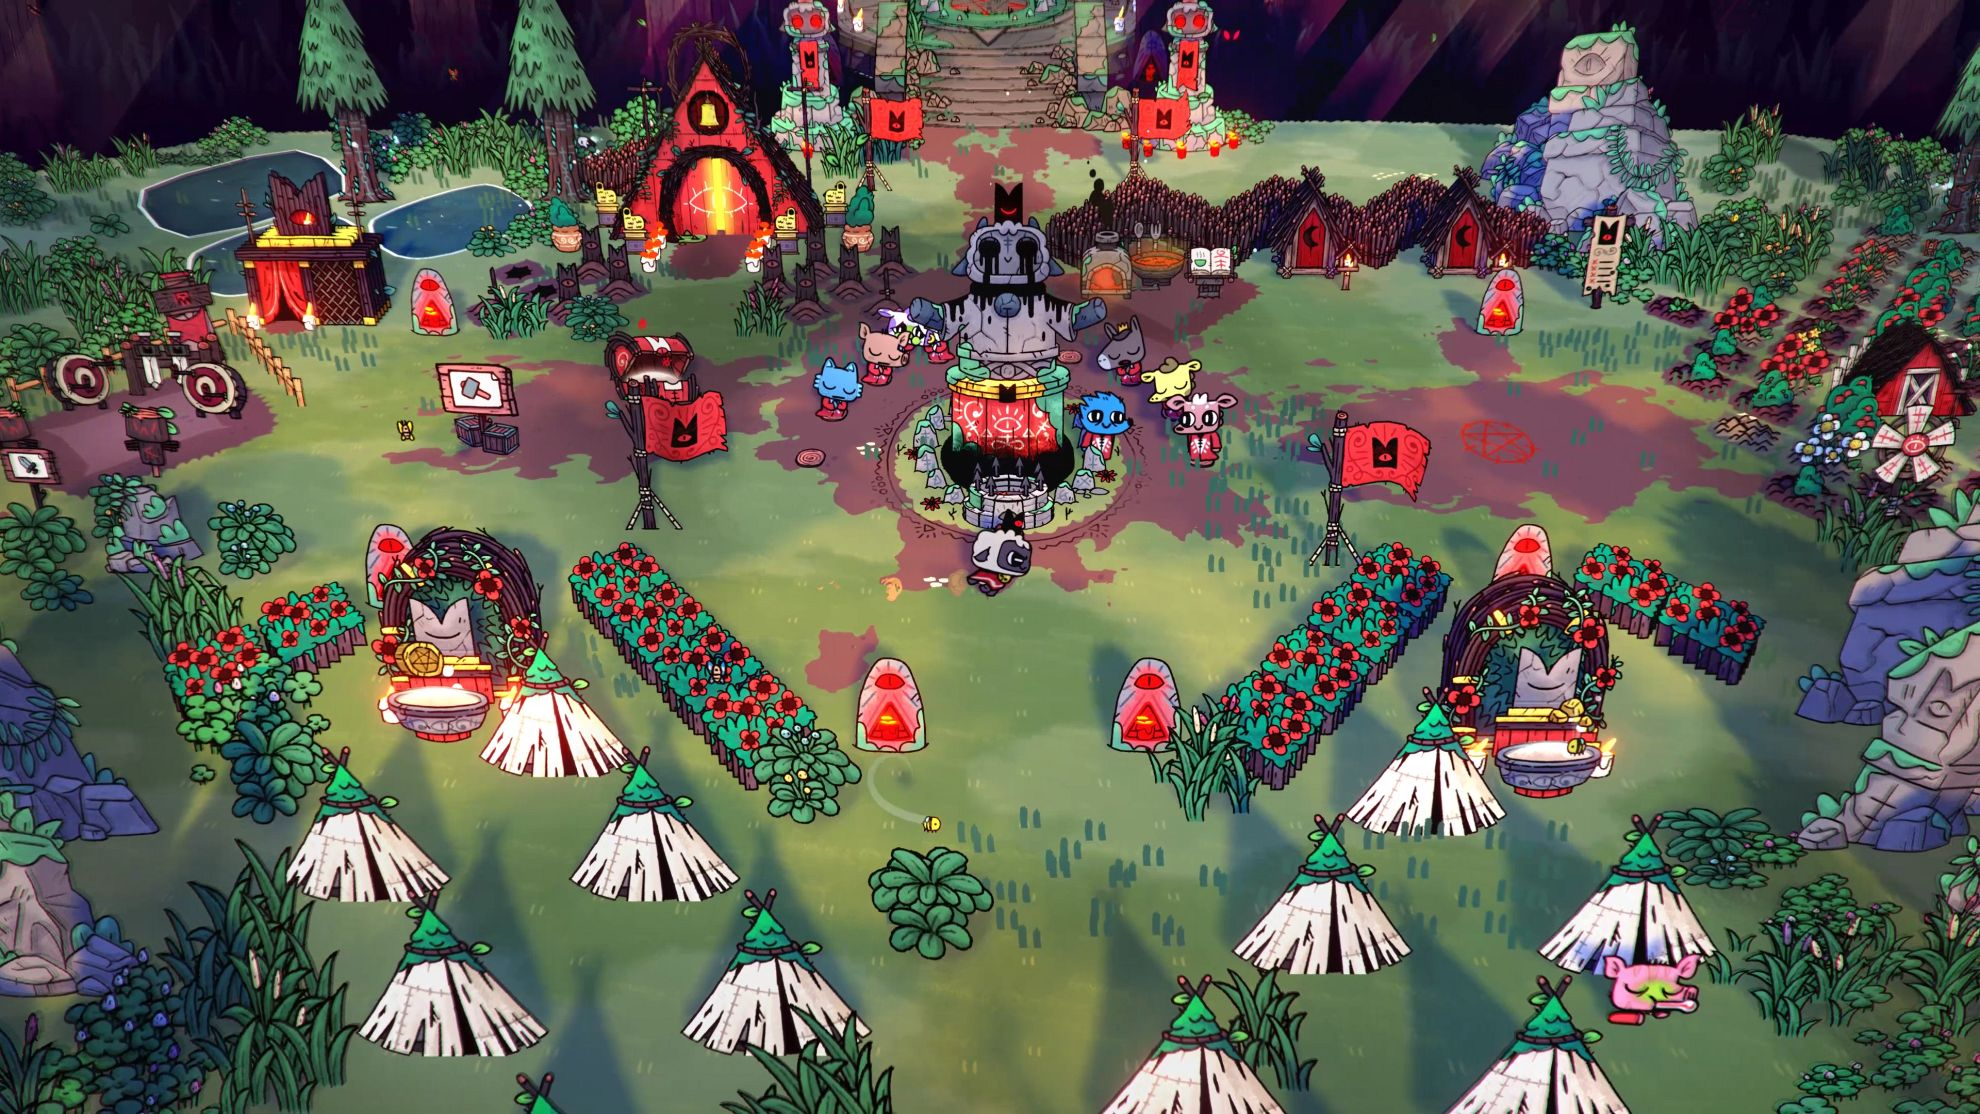
\includegraphics[width=350px,clip=true]{cult_of_the_lamb.png}
    \caption{Cult of the Lamb}
    \label{fig:clamb}
\end{figure}

\subsection{Herramientas de Movimiento de Personajes}
En la Unity Asset Store\cite{unityAssetStore} es muy común encontrar paquetes que incluyan controladores de personajes de distintos tipos. Lo normal es que permitan unicamente un tipo de movimiento concreto ajustado
 a un tipo de cámara, si el espacio es 2D o 3D o si el movimiento está regido por físicas o no. En algunos casos, como el de Easy Character Movement 2\cite{ECM2} si que se incluye un entorno más genérico que permite,
 con trabajo adicional, contar con algunas (o todas) las combinaciones de los factores mencionados anteriormente. En el caso de DUJAL, sin embargo, se quieren implementar todas las combinaciones posibles de dichos 
 factores de antemano con el objetivo de tener el completo abanico de posibilidades de movimiento sin necesidad de trabajo adicional por parte del usuario, además de expandir las funcionalidades que se suelen 
 definir estándar, como por ejemplo la posibilidad del 'Wall Running'\cite{wallRun}, 'Wall Jumping'\cite{wallJump} o 'Dashing'\cite{dash}.

\subsection{Herramientas de Generación de Mazmorras}
Respecto a las herramientas de generación de mazmorras al igual que ocurre con las de sacudida de cámara, no parece que haya demasiadas opciones. La más relevante sería Procedural Dungeon 
Generator\cite{ProceduralDunGen}, que permite la generación de mazmorras del estilo Dungeon Crawler o Roguelike de forma procedimental dados unos parámetros de entrada (Como tamaño, numero de salas, tipos de sala etc...).
Del mismo modo, el Generador de Mazmorras de DUJAL permite algo muy similar, con el añadido de permitir además generar laberintos usando un algoritmo muy similar.

\subsection{Resumen del Estado del Arte}
Como queda patente en esta sección, en lo referente a herramientas auxiliares al desarrollo de videojuegos hay una infinidad de opciones que usar, y aunque puedan haber opciones mejores, peores, más caras o más baratas,
es muy difícil que una en concreto se ajuste a un caso de uso particular, las opciones se reducen siempre a invertir un tiempo significativo en adaptar el juego que se esté desarrollando a una ya existente, o por el contrario, 
crear la herramienta de cero. El código del que se compone DUJAL pretende ser fácilmente escalable para poder ajustar la herramienta al juego, en lugar de al revés, para intentar lidiar con ese roce que tiende a ocurrir al 
buscar herramientas externas al motor.